%%%%%%%%
\chapter{Methods and Materials}

\section{Ethical approval}
The Ethics Committees at the University of British Columbia approved all the experiments using human resources. Patients in Vancouver, British Columbia, undergoing excision or diagnostic core biopsy were recruited, and samples were collected after written consent, under the tumour tissue repository (TTR-H06-00289) protocol and transplanted in mice under the Neoadjuvant patient derived xenografts (PDX) (University of British Columbia BC Cancer Research Ethics Board H20-00170) protocols. All experimental methods comply with the Helsinki declaration. All animal studies were approved by the Animal Care Committee at the University of British Columbia.  


\section{Establishment of patient derived xenografts} 
Patient's tumor materials were processed as described in \cite{eirew2015dynamics} and transplanted in mice under the \ac{ARC} bioethics protocol (A19-0298-A001) approved by the animal care committee.
Briefly, tumour fragments were chopped finely with scalpels and mechanically disaggregated for one minute using a Stomacher 80 Biomaster (Seward Limited, Worthing, UK) in \SIrange{1}{2}{\ml} cold DMEM/F-12 with Glucose, L-Glutamine and HEPES (Lonza 12-719F).
An aliquot of \SI{200}{\ul} of medium (containing cells/organoids) from the resulting suspension was used equally for 4 transplantations in mice.

Tumours were transplanted in mice as previously described~\cite{eirew2015dynamics} in accordance with SOP BCCRC 009. 
Briefly, female immuno-compromised, NOD/SCID/IL2r$\gamma^{\small{-/-}}$\ac{NSG} and        
\ac{NRG} \cite{pearson2008non} mice were bred and housed at the animal resource centre \ac{ARC} at the British Columbia (BC) Cancer Research Centre . 
For subcutaneous transplants, mechanically disaggregated cells and clumps of cells were re-suspended in \SIrange{150}{200}{\ul} of a 1:1 v/v mixture of cold DMEM/F12: Matrigel (BD Biosciences, San Jose, CA, USA).
8-12 weeks old mice were anesthetized with isofluorane, then the mechanically disaggregated cells/clumps suspension was injected under the skin on the left flank using a \SI{1}{\ml} syringe and 21gauge needle. 
The animal care committee and animal welfare and ethical review committee, the University of British Columbia (UBC), approved all experimental procedures.

\subsection{Histopathology of PDX tumours} 
The hormone receptor status of most of the tumour samples was determined by immunohistochemistry and FISH (Fluorescence in situ hybridization) copy number.
Two separate tissue microarrays were prepared using duplicate \SI{1}{\mm} cores extracted from formalin-fixed paraffin-embedded blocks containing material from all passages of the patient derived xenografts (3 TNBC and HER2+) used for this project. 
Deparaffinized \SI{4}{\um} sections of paraformaldehyde fixed tumours were processed for immunohistochemistry (IHC) using a Discovery XT automated system (Ventana Medical Systems, Tucson, AZ, USA). 
EGFR, INPP4B, Ki67, PR, ECAD were all performed on the Ventana Discovery XT platform using CC1 for antigen retrieval, incubating for one hour at room temp, and using the UltraMap DAB detection kit.
Primary antibodies to ER$\alpha$ (clone SP1, Ventana), HER2 (clone 4B5, Ventana), EGFR (clone EP22, Epitomics, Burlingamen, CA, USA) and Ki67 (clone SP6, Thermo Scientific) 
Horseradish peroxidase-conjugated Discovery Universal Secondary Antibody (Ventana) was then applied and the slides developed using 3,3’-diaminobenzidine Map Kit (Ventana). 
The slides were reviewed by a pathologist. Representative images from SA609 TNBC and HER+ PDX early and late passages are shown in \textbf{\autoref{fig:HistologyHER2+TNBC}}. These images indicates that in our PDX model system, the tumors retain architecture and receptor markers from early to late passages.


 \begin{figure}
\centering
\includegraphics[width=\textwidth]{Figures/HistologyHER2+TNBC.pdf}
	
\caption[Untreated PDX timeseries and growth trajectories]
	{\small
\textbf{Representative patterns of expression on histology in early and late passages.}
 \textbf{(a)}, IHC of HER2+ tumours at passage 1 (X1) and passage 10 (X10), 4x and 20x (insets). Scale bars \SI{500}{\micro\metre} and \SI{100}{\micro\metre} (insets). On top of each panel presenting the antibody name and the right bottom square is showing the score of the stain.
\textbf{(b)} IHC of TNBC SA609 tumors at passage 2 (X2) and passage 10 (X10), 4x and 20x (insets). Scale bars \SI{500}{\micro\metre} and \SI{100}{\micro\metre} (insets). On top of each panel presenting the antibody name and the right bottom square is showing the score of the stain.}
	\label{fig:HistologyHER2+TNBC}
\end{figure}


Sections were deparaffinized in xylene, rehydrated in graded alcohol, and used for histology and immunostaining. 
H \& E and \ac{IHC}  of the two PDX tumours showed that TNBC is  derived from a triple negative breast cancer patient while HER2+ was derived from a HER2+ breast cancer patient. HER2 IHC was scored as 2+, HER2/CEP17 ratio was calculated as 6.5 (positive)\cite{ahn2020her2} from  \ac{FISH}  and focal high level amplification (average copy number state of 10) of the \ac{ERBB2} locus (approximately Chr17:37500001-38000000) was found in the DLP+ data.

\begin{table}
\centering
\caption{List of antibodies and experimental conditions.}
Summary of antibodies clones and their suppliers used for staining TMAs for IHC.

\small\textbf{(*RTU: Ready to use; N/A: not applicable)}.
\label{stab:antibodieslist}
\begin{tabular}{|rl|l|l|l|}
  \hline
 & Specimen & Stain/IHC & Vendor / Ab Clone & Dilution  \\ 
  \hline
1 & TMA1 \& 2 & CK14 & Empire Genomics clone LL002 & 1 in 50 \\ 
  2 & TMA1 \& 2 & Ck5/6 & Dako D5/16 B4 & *RTU  \\ 
  3 & TMA1 \& 2 & Ck8 (CAM5.2) & BC Bioscience CAM5.2 & 1 in 10  \\ 
  4 & TMA1 \& 2 & EGFR & Epitomics 1902-1 & 1 in 100  \\ 
  5 & TMA1 \& 2 & ER & Ventana  clone SP1 & *RTU\\ 
  6 & TMA1 \& 2 & H\&E & *N/A & *N/A \\ 
  7 & TMA1 \& 2 & INPP4B & Abcam EPR3108Y ab81269 & 1 in 50 \\ 
  8 & TMA1 \& 2 & Ki67 & Abcam ab16667  & 1 in 400  \\ 
  9 & TMA1 \& 2 & PR & Abcam ab30285 & 1 in 200  \\ 
  10 & TMA1 \& 2 & Slug/Snail & Abcam ab85936 & 1 in 125 \\ 
  11 & TMA1 \& 2 & SMA & Dako clone 1A4 & 1 in 100 \\ 
  12 & TMA1 \& 2 & Trichrome & Sigma-HT15-1KT & *N/A \\ 
  13 & TMA1 \& 2 & Twist & NB120-49254 & 1 in 200\\ 
  14 & TMA1 \& 2 & Vimentin & Dako V9 & RTU  \\ 
  15 & TMA1 only & E-Cad & Cell Signal 3195 & 1 in 100  \\ 
  16 & TMA1 only & HER2 & Roche 4B5 & 1 in 8  \\ 
  17 & TMA2 only & E-Cad & Dako NCH-38 & *RTU  \\ 
  18 & TMA2 only & HER2 & Ventana  clone 4B5 & *RTU \\ 
   \hline
\end{tabular}%
\end{table}

\subsection{Serial passaging of PDX}
Tumours were serially passaged as  described \cite{eirew2015dynamics}.
Briefly, for serial passaging of PDX, xenograft-bearing mice were euthanized when the size of the tumours approached \SI{1000}{\mm\cubed} in volume (combining together the sizes of individual tumours when more than one was present).
The tumour material was excised aseptically, then processed as described for primary tumour. 
Briefly, the tumour was harvested and minced finely with scalpels then mechanically disaggregated for one minute using a Stomacher 80 Biomaster (Seward Limited, Worthing, UK) in \SIrange{1}{2}{\ml} cold DMEM-F12 medium with Glucose, L-Glutamine and HEPES. 
Aliquots from the resulting suspension of cells and fragments were used for xenotransplants in next generation of mice and cryopreserved.
Serially transplanted aliquots represented approximately 0.1-0.3\%  of the original tumour volume. HER+ and TNBC PDX were passaged upto 10 generations and scWGS was carried out at each timepoint while scRNAseq was done at initial, mid and late timepoint. 

\subsection{TNBC PDX tumour mixing experiments} Frozen untreated passages three (X3) and eight (X8) vials from TNBC PDX, were thawed and  physically remixed in two different volumetric proportions of X3:X8 by tumour weight at the ratio of approximately 1:1 and 1:0.4, labelled as mixture branch a and branch b, respectively. From each of different dilutions, \SI{200}{\ul} of aliquot was taken to be used to transplant in two mice each using the same protocol of transplantation as described above. Before transplantation a small proportion of the physical mixture of cells, from the 1:1 ratio, was subjected to whole genome single cell sequencing to measure the baseline clonal composition labelled as M0 and its subsequent PDX as M1 \textbf{\autoref{fig:Mixturenew} a)}. Each of the thawed X3 and X8 cell populations used for mixing were also transplanted independently to confirm the viability of the tumour material for PDX tumour growth. The tumour cell mixture was then serially passaged over 4 generations, designating the transplants as M1-M4. Tumours from each X3:X8 serial passages from both mixture branches were collected and analysed with scWGS (DLP+) as for other samples.

\subsection{TNBC PDX timeseries treatment with chemotherapies}
\label{ssec:rx}
NRG mice of the same age and genotype as above were used for transplantation treatment experiments. Drug treatment with cisplatin (Platinum) was commenced when the tumour size reached approximately \SIrange{300}{400}{\mm\cubed}. Cisplatin (Accord DIN: 02355183)  was administered i.p. at \SI{2}{\mg\per\kg} every third day for 8 doses maximum (Q3Dx8). The dosage schedule was adjusted 50\% less than what is mentioned in the literature \cite{li2013enhanced,wang2013klotho} and around one third of the maximum tolerated dose (MTD) calculated in the immunodeficient mice  \textbf{(\autoref{fig:treatmentdesignMTD} b)} . Low dose cisplatin pulse and tumour collection timings were optimized to achieve the experimental aims of tumour resistance. The aim was to collect tumour at 50\% shrinkage (from the starting tumour at the time treatment started) in size when measured with a caliper. Cisplatin \SI{1}{\mg\per\ml} was diluted in 0.9\% NaCl to obtain concentrations \SI{200}{\ul}/\SI{20}{\g} of mouse weight and kept in glass vials at room temperature. Quality control \ac{QC} samples were prepared freshly on each day prior to the dosing. Mice were continually monitored for acute signs of toxicity including pain at injection site, skin tenting, coat scruffing, sunken eyes, food consumption and behaviour for the first two hours following compound administration. For TNBC PDX, 8 mice at initial passage were transplanted in parallel for the treatment/treatment holiday study group. Half of the mice were treated with cisplatin when tumours exhibited around 50\% shrinkage, the residual tumour was harvested as above and re-transplanted for the next passage in the group of eight mice. Again, half of the mice at X5 were kept untreated while the other half were exposed to cisplatin following the same dosing strategy. Four cycles of cisplatin treatment were generated, with a parallel drug holiday group at each passage. Cisplatin treated tumours were coded as \textit{UT, UTT, UTTT, UTTTT} for each of the four cycles of drug respectively, while the tumours on drug holiday were labelled as \textit{UTU, UTTU} and \textit{UTTTU} for the three timepoints. Each number of \textit{T} exhibits the number of cycles of drug exposure. SA535 TNBA PDX was also treated with CX5461, the same way like cisplatin. CX-5461 was dissolved in 50mM NaH2PO4, pH4 for xenograft application. CX-5461 was administered through oral gavage once every three days at the final dose of \SI{50}{\mg\per\kg}.
Sc-WGS and scRNAseq was carried out from each tumour during the timeseries treatment with counterpart drug holiday and untreated controls  \textbf{(\autoref{fig:treatmentdesignMTD} a)}.

\begin{figure}
\centering
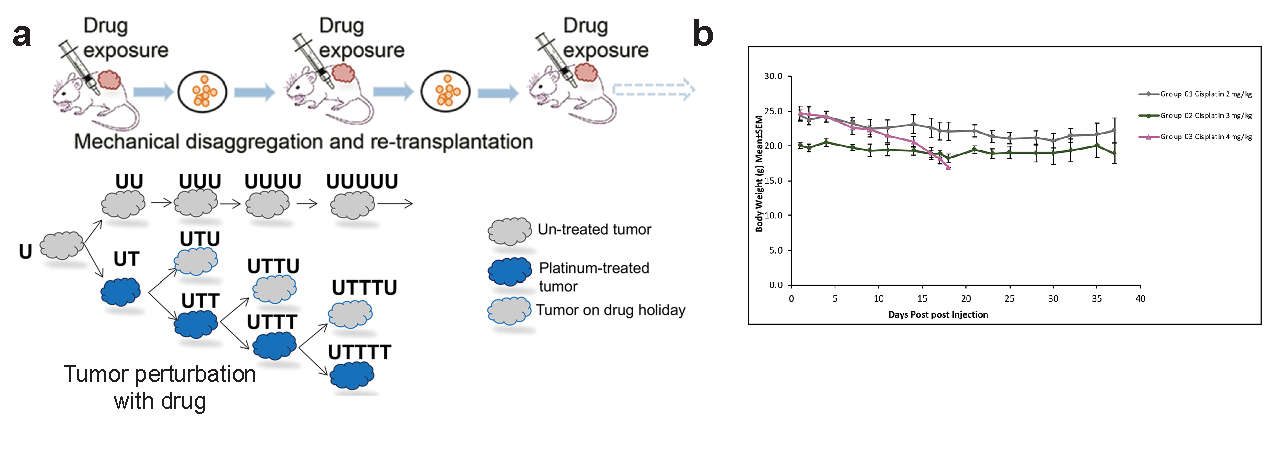
\includegraphics[width=\textwidth]{Figures/treatmentdesignMTD.pdf}
	
\caption[Experimental overview of TNBC PDX treated time series]
	{\small
	\textbf{Experimental overview of treatment design in TNBC PDX time series}
\textbf{(a)} Experimental design of cisplatin treatment in PDX.The residual tumour from one treated mouse was re-transplanted in the next (n=8). The solid blue colour represent cisplatin treated tumours \textit{(UT, UTT, UTTT, UTTTT)}; blue outlined in grey represents drug holiday \textit{(UTU, UTTU, UTTTU)}. Grey represent the untreated series \textit{(U, UU, UUU, UUUU, UUUUU)} \textbf{(b)} Mouse body weight graph recorded during \ac{MTD} evaluation of cisplatin in NRG mice (n=3 in each study cohort).}
	
	\label{fig:treatmentdesignMTD}
\end{figure}


\subsection{PDX tumour growth measurement curves} 
NRG mice received sub-cutaneous inoculation (SQ) of tumour cells (\SI{150}{\ul}) on day 0. 
The tumours were allowed to grow to palpable solid nodules.
Around 7-9 days after they are palpable, their size were measured with calipers every 3rd day. 
tumours were measured in two dimensions using a digital caliper and expressed as tumour volume in mm3; defined as: [volume= 0.52$\times$(Length)$\times$(Width)].
Under drug perturbation, the treated tumours in the first two cycles of treatment showed rapid growth reduction but in third cycle started showing non-responsive behaviour leading to total resistance in fourth cycle 



\section{PDX tumor dissociation into single cells}

\subsection{Tissue dissociation at 37\textdegree C}
Tumour fragments from patient breast and ovarian samples and PDXs were incubated for 2 hrs with a collagenase/hyaluronidase enzyme mix in serum-free Dulbecco's Modified Eagle's Medium (DMEM) at 37\textdegree C with intermittent gentle trituration with a wide bore pipette tip. Cells were resuspended in 0.25\% trypsin-edta for 1 min followed by neutralization with 2\% FBS in Hank's Balanced Salt Solution (HBSS) and centrifugation. Cells were resuspended in 2\% FBS/HBSS and filtered through a 40\textmu m filter. Where necessary, dead cells were removed using MACS Dead Cell Removal Beads (Miltenyi Biotec) according to the manufacturer's instructions. Cells were centrifuged and resuspended in 0.04\%  BSA/PBS and cell concentration adjusted for scRNAseq. For timecourse experiment, tissue was dissociated as above for 3 hrs with samples taken at 30 mins, 1 hr and 2 hr.

\subsection{Tissue dissociation at 6\textdegree C}
Tumour fragments were incubated for 30 minutes at 6\textdegree C with a serine protease, subtilisin A, derived from the Himalayan soil bacterium \textit{Bacillus Lichenformis} (Creative Enzymes NATE0633) in PBS supplemented with 5mM CaCl2 and 125U/ml DNAse, as described in \cite{adam2017psychrophilic, potter2019dissociation}. During dissociation, samples were gently triturated every 5 minutes using a wide-bore pipette. Cells were resuspended in 0.25\% trypsin-edta for 1 minutes at room temperature, neutralized with 2\% FBS in HBSS and filtered through a 40\textmu m filter. Following dissociation, samples were processed for scRNAseq as described above. For the timecourse experiment, tissue was dissociated as above for 3 hours with samples taken at 30 minutes, 1 hour and 2 hours. 

\subsection{Removal of murine contamination from patient derived xenograft samples}

To identify murine cells in the PDX samples, we re-ran CellRanger version 3.0.2 aligning cells to both GRCh38 and mm10 (separately). We then considered all cells for which a valid barcode was identified in the raw (unfiltered) data for either alignment, and counted the number of reads mapping to each genome for each cell. A cell was subsequently designated as a contaminating mouse cell if more reads mapped to mm10 than GRCh38, and a human cell otherwise.

\section{\textit{in vitro} cultures and assays}

\section{chemotherapies}
For \textit{in vitro} assays, the chemotherapies used are summarized in table.


\subsection{WST-1 assay}
In all the experiments in \textbf{\autoref{fig:invitro}}, the cell viability was measured by WST-1 assay according to the protocol provided by manufacturer (Roche, Catalogue number 11644807001). Single cells from PDX and Wild type and HCT116 (DNA-PK and Lig4 knockout) cells were plated in 96-well plates either untreated or treated with drug continuously during the indicated time before WST-1 assay. Drug incubation time was 6-7 days. Absorbance was read with the microplate reader SpectraMax 3 (Molecular Devices, Sunnyvale, CA, USA).

\subsection{Dose response curve fitting for cell line WST-1 assay}
Where sigmoid curves were appropriate for dose response analysis, a four-parameter logistic regression curve was fitted to the data using the R function ‘nlme’. An IC50 was estimated, the difference in IC50 values was calculated for conditions with and without drug. The set of differences was tested using the Student's paired t-test.

\section{Live/dead cells analysis}

\subsection{Flow Cytometry for live/dead cells staining}
 GM18507 cells were treated with or without 100ng/ml TNF\textalpha for 24 hours before being stained with propidium iodide (catalogue no.P1304MP, Theromofisher scientific) and FITC annexin V (catalogue no.640905, Biolegend) and sorted into dying, dead or live populations according to single, double or negative staining respectively using a FACS Aria Fusion (BD Biosciences).
 
\subsection{Clustering of live, dying, and dead cells}
Cells were hierarchically clustered using the \texttt{hclust} function in \texttt{R} applied to the 10-dimensional output of MNN, and clusters assigned using the \texttt{cutree} function.

\subsection{Reproducible data analysis}
A dockerized workflow to enable reproduction of all figures and analysis in this paper is available (Campbell, K. kieranrcampbell/scrnaseq-digestion-paper. Github. \url{https://github.com/kieranrcampbell/scrnaseq-digestion-paper}(2019). Corresponding docker image is at \url{https://cloud.docker.com/u/kieranrcampbell/repository/docker/kieranrcampbell/statgen2} (version 0.4).

\section{Single cell whole genome sequencing and library construction with DLP+}

All libraries, including metrics on number of cells, average number of reads per cell and quality control metrics are listed in refsuptab{tab:omnibusMedians}.

\subsection{Creation of single cell suspensions from PDX}
Tumour fragments from PDX samples were incubated with a collagenase/hyaluronidase 1:10 (10X) enzyme mix (STEM CELL technologies, Catalog \#07912) in  \SI{5}{\ml} DMEM/F-12 with Glucose, L-Glutamine and HEPES (Lonza 12-719F)and 1\%BSA at \SI{37}{\degreeCelsius} with intermittent gentle pipetting up and down the sample every 30 min for 1 min, during the first hour with a wide bore pipette tip, and every 15-20 min for the second hour, followed by  centrifugation (1100 rpm, 5 min) and supernatant removal.
The tissue pellet was resuspended in \SI{1}{\ml} of  0.25 percent trypsin-EDTA (VWR CA45000-664) for 1 min, superadded by \SI{1}{\ml} of DNAse 1/dispase \SI{100}{\ul}/\SI{900}{\ul} (StemCell 07900,00082462) pipetted up and down 2 min, followed by neutralization with 2\% FBS in HBSS with 10 mM HEPES (STEMcells Catalog \#37150). 
This cell suspension was then passed through a \SI{70}{\micro\metre} filter to remove remaining undigested tissue and centrifuged for 5 min at 1100 rpm after topping it up to \SI{5}{\ml} with HBSS.
Single cells pellet  was resuspended in PBS + 0.04\% BSA (Sigma) in appropriate volume to achieve  $\approx$~1 million per ml concentration of cells for robot spotting for DLP+.

\subsection{Robot spotting of single cells into the nanolitre wells and library construction}
scWGS DLP+ library construction was carried out as described in \cite{laks2019clonal}. Briefly, single cell suspensions from cell lines and patient derived xenografts were fluorescently stained using CellTrace CFSE (Life Technologies) and LIVE/DEAD Fixable Red Dead Cell Stain (ThermoFisher) in a PBS solution containing 0.04\% BSA (Miltenyi Biotec 130-091-376) incubated at \SI{37}{\degreeCelsius} for 20 minutes. Cells were subsequently centrifuged to remove stain, and resuspended in fresh PBS with 0.04 percent BSA. This single cell suspension was loaded into a contactless piezo electric dispenser (sciFLEXARRAYER S3, Scienion) and spotted into the open nanowell arrays (SmartChip, TakaraBio) preprinted with unique dual index sequencing primer pairs. Occupancy and cell state were confirmed by fluorescent imaging and wells were selected for single cell copy number profiling using the DLP+ method \cite{laks2019clonal}. Briefly, cell dispensing was followed by enzymatic and heat lysis. After cell lysis, tagmentation mix 
(\SI{14.335}{\nano\liter} TD Buffer, \SI{3.5}{\nano\liter} TDE1, and \SI{0.165}{\nano\liter} 10\% Tween-20) in PCR water were dispensed into each well followed by incubation and neutralization. Final recovery and purification of single cell libraries was done after 8 cycles of PCR. Cleaned up pooled single-cell libraries were analyzed using the Aglient Bioanalyzer 2100 HS kit. Libraries were sequenced at UBC Biomedical Research Centre (BRC) in Vancouver, British Columbia on the Illumina NextSeq 550 (mid- or high-output, paired-end 150-bp reads), or at the GSC on Illumina HiSeq2500 (paired-end 125-bp reads) and Illumina HiSeqX (paired-end 150-bp reads). The data was then processed to quantification and statistical analysis pipeline \cite{laks2019clonal}.

\section{Single cell whole genome data analysis}
\subsection{DLP+ sequence analysis, copy number determination and quality control filtering}
FASTQ pre-processing, sequence alignment, quality control, copy number calling and S-phase classification and filtering was performed on all libraries as detailed in \cite{laks2019clonal}. Briefly, cells were assigned a quality score (QS) for data quality based on a 13 feature Random forest classifier fitted and applied as per \cite{laks2019clonal}. Copy number alterations on a per cell basis were determined using a hidden Markov Model (HMM) approach using the \texttt{HMMCopy} package with parameterizations detailed in \cite{laks2019clonal}. S-phase cells were identified using an automated classifier trained using cell-cycle sorted cells and where features from HMM output were used to identify cells most probably in early or late phase replication of their genomes. As these cells interfere with downstream phylogenetic analysis, they were removed from the analysis according to parameter settings and thresholds established in \cite{laks2019clonal}. To further enable phylogenetic inference, 10-15\% of cells with highest average copy number state jumps were removed. Upon inspection, these cells included early and late dividing cells that were not captured by the s-phase classifier. 
Attrition of cells at each stage of quality control is shown in (suptabtab:omnibusMedians).



\subsection{Identifying clones through phylogenetic analysis}
Using sitka we established the evolutionary relationships of cells in a PDX heterogeneous samples. To investigate cancer evolution we need to determine the abundance of subpopulations over time. To this end, we introduce \texttt{Lumberjack}, a tree-cutting algorithm that we used to define clonal subpopulations. In the output tree of \texttt{sitka}, cells are part of the terminal leaf nodes of the phylogenetic topology. We post-processed the inferred trees to identify clonal populations from major clades. When clonal populations are defined, their abundances were counted as a function of timeseries and these were used for fitness inference. 
Clones are constructed by identifying connected components (each a clade or a paraphyly) in the phylogenetic tree reconstruction. The tree is `cut' into discrete populations according to the following procedure

\subsection{Phylogenetic tree inference, clone determination and clonal abundance measurements}

We developed a single cell Bayesian tree reconstruction method based on copy number change point binary variables called \texttt{sitka} \cite{dorri2020efficient} to fit phylogenetic trees to the copy number profiles.  
In the output of \texttt{sitka}, cells are the terminal leaf nodes of the phylogenetic topology.  
The inferred trees were post-processed to identify clonal populations from major clades. With clonal populations defined, their abundances were counted as a function of timeseries and these were used for fitness inference (see below). 
Clones were constructed by identifying connected components (each a clade or a paraphyly) in the phylogenetic tree reconstruction. The tree was `cut' into discrete populations according to the following procedure (see Algorithm \cite{salehi2020single}).
%%Notation
Let $L$ be a set of loci and $C$ a set of cells and ${\lvert}L{\rvert}$. 
Define $\tau = (L, C, E)$ to be a rooted phylogenetic tree with $E$ its set of directed edges.
The phylogenetic tree is assumed to comprise internal nodes that are phylogenetic markers (loci) and terminal nodes that are either cells or loci. 
Terminal loci are considered unused phylogenetic markers and are discarded. 
Let ${\lvert}\tau{\rvert} = {\lvert}C{\rvert}$, that is the number of cells that belong to tree $\tau$.
By $\tau_{l} = (L_l, C_l, E_l)$ denote the subtree rooted at node $l$.
Set $\text{pa}(l)$ and $\text{child}(l)$ be the parent node and set of immediate children of node $l$ with $\text{desc}(l)$ comprising all its descendant. 

% Final clone determination
The inputs to the algorithm are the rooted phylogenetic tree $\tau$ and the copy number states of its cells.
A clone is defined as connected components (each a clade or a paraphyly) in the graph tree $\tau$ composed of cell of sufficient genomic homogeneity. 
The degree of homogeneity can be tuned by limiting the number of loci and the difference in copy number of sub-clades in a clone. 
The algorithm works by first finding the coarse structure, that is dividing the tree into major clades and then looking for fine structures within each clade by traversing the tree in a bottom up manner and merging loci that are sufficiently similar.
The remaining loci constitute the roots of detected clades.

% First pick coarse structures
To obtain the coarse structure from the reconstructed phylogenetic tree we use a two step procedure. (i) First we identify monophyletic clades via algorithm \cite{salehi2020single}. 
(ii) We then remove the cells comprising the clades found in step one from the tree and repeat algorithm. 
We note that these new clades (if any) could be paraphyletic.

To find the fine structures within the initial clades we use the following procedure.
For each clade and its corresponding sub-tree $\tau_s$, denote by $L_s$ a set of loci $l$ for which $m \le \lvert \tau_l \rvert \le M$. 
In a bottom-up traverse of the tree, for each node $l \in L_s$, remove it from $L_s$ if $\lvert \tau_{\text{pa}(l)} \rvert - \lvert \tau_{l} \rvert \le n$, otherwise remove $\tau_{l}$ from $\tau_c$
At the end of the tree traversal set $L_s$ contains new candidate roots for each initial clade.
For each $l \in L_s$ define the summary copy number profile as a vector whose $i$th element is the median of the copy number states of the $i$th for all cells in $\tau_{l}$.
Compute the distance between two subclades as the mean absolute difference of their median genotypes.
Merge subclones induced by $L_s$ if their summary copy number profiles are too similar.
We can do this by computing a t-test over the pairwise distances to exclude outlier subclades and merge the rest. we opted to also split clades by the ploidy of their constituent cells, where ploidy is defined as the most recurrent CN state in the cell.  

%A cut at a locus in the tree is defined as the trajectory induced by the subtree %rooted at the base node of that locus, i.e., the node farthest from the root.
%A locus that meets all the conditions above is called an eligible locus.
Once clones are identified, we set the abundance of each clone at a specific timepoint as the fraction of cells in that clone from that timepoint.
For estimation of clonal fractions, we used the following procedure (i) let $M$ denote the mutational cellular prevalence (rows) estimated over multiple timepoints (columns) using the multi-sample \texttt{PyClone}~\cite{roth2014pyclone} model, (ii) define $A$ as the genotype matrix (which mutation-cluster (rows) is present in which clones (columns), (iii) then we set $A X = M$ where $ X = A^{-1}M$ are the clonal fractions overtime. (iv) we solve for $X$ using QR-decomposition.


\section{Single cell RNA sequencing (scRNAseq)}

\subsection{Processing of patient derived xenografts for scRNAseq data}
PDX tumours were harvested and mechanically disaggregated into small fragments to viably freeze them according to the protocol mentioned above. 
One of the viable frozen tumour vial was thawed and after washing out the freezing media, the tumour clumps and fragments were incubated with digestion enzymes as with DLP+ preparation. After complete dissociation with collagenase/hyaluronidase enzyme mix according to the protocol at \SI{37}{\degreeCelsius}, followed by briefly washing in 0.05\% trypsin-EDTA and resuspension in 0.04\% BSA in PBS. Dead cells were removed using the Miltenyi MACS Dead Cell Removal kit and cells were processed as previously described \cite{o2019dissociation}.
To avoid processing artifacts, dissociation methods and times were tightly controlled and for treatment and treatment holiday pairs, library construction was performed on the same chips. Single cell suspensions were loaded onto the 10x Genomics single cell controller and libraries prepared according to the Chromium Single Cell 3’ Reagent Chemistry kit standard protocol. 
Libraries were then sequenced on an Illumina Nextseq500/550 with 42bp paired-end reads, or a HiSeq2500 v4 with 125bp paired-end reads. 10x Genomics Cell Ranger version 3.1 was used to perform demultiplexing,  counting and alignment to GRCh38.

\subsection{Quality control}

Count matrices were generated using CellRanger version 3.1.0. Cells were considered to have passed a quality control filter (QC-filter) and retained for subsequent analysis if they met the following criteria: (i) at least 1000 genes detected, (ii) less than 20\% of counts (UMIs) mapping to genes from the mitochondrial genome (``mitochondrial genes''), (iii) fewer than 60\% of counts (UMIs) mapping to ribosomal genes, and (iv) the total counts (UMIs) per cell was at most 3 median absolute deviations lower than the overall median. Cells not matching all criteria were filtered using the \texttt{calculateQCMetrics} and \texttt{isOutlier} functions in the \texttt{scater} package \cite{mccarthy2017scater}. Then, all the mouse cells were eliminated. A cell is called a mouse cell if the total number of counts in a mouse alignment of the 10x sample was greater than the total number of counts in a human alignment. Finally, we eliminated doublets using package \texttt{scrublet} \cite{scrublet}.

\subsection{Gene expression normalization}

Sample level normalized log expression values were computed using \texttt{scran} \cite{lun2016pooling} with grouping variables calculated from clustering using the \texttt{quickCluster} function \cite{lun2016step}. Overall normalized expression was computed by merging sample level matrices and recalculating normalized expression with grouping labels computed on the merged matrix. Batch correction between libraries was performed using Scanorama \cite{hie2019efficient} on the overall normalized expression values with default parameters and the library id as the batch label.

\subsection{Dimensionality reduction}

Principal component analysis was performed on the batch corrected expression matrix using the \texttt{scater} \cite{mccarthy2017scater} R package.  A single two dimension UMAP \cite{becht2019dimensionality} embedding was generated using the first 50 principle components. This embedding was used in downstream analysis and visualizations.

\subsection{Pathway Enrichment Networks}

Enriched pathways were computed from differentially expressed genes (adjusted p-value $<$ 0.01) ranked by log fold change.  A normalized enrichment score (NES) was calculated from a ranked gene set enrichment analysis (GSEA) \cite{shi2007gene} performed on each subset of differentially expressed genes using the hallmark gene set collection from MSigDB \cite{liberzon2015molecular}.  Significantly enriched pathways (adjusted p-value $<$ 0.01) and pathway specific differentially expressed genes were included in network enrichment figures.  
Pathway nodes were colored by NES value. Edges are defined between pathways sharing genes.
All analysis and visualization was performed using \texttt{gseapy} and \texttt{networkx} \cite{hagberg2008exploring} Python packages.

\subsection{Integrative genome-transcriptome analysis with \texttt{clonealign}}
\texttt{clonealign} version 1.99.2 was used to align scRNAseq cells to the DLP+ clones obtained. First, genes whose purity was less than 60\% in any clone (40\% for \textit{X5 UT}) were removed, where the purity of a gene in a clone  is defined as the percentage of cells that have the modal copy number for that gene and clone. Then, we used the following clonealign parameters: \texttt{n\_repeats = 3}, \texttt{mc\_samples = 1}, \texttt{learning\_rate = 0.07}, \texttt{max\_iter = 500}, \texttt{data\_init\_mu = TRUE} for all samples except \texttt{FALSE} for \textit{X5 UTU}, \texttt{data\_init\_mu = FALSE},
\texttt{saturation\_threshold = 6} and \texttt{clone\_call\_probability = 0.9}.

\section{Differential expression analysis}

\subsection{Differential expression of temperatures and core heat-related gene set} 

All differential expression analyses were performed with edgeR \cite{robinson2010edger} version 3.24.3 using the quasi-likelihood F-test as was the top-performing method in a recent review \cite{soneson2018bias}. We included the patient / xenograft / cell line ID in the design matrix to account for unwanted technical and biological variation. In every case we only considered genes with minimum 10 counts across all cells.
We defined the core set of genes as those with FDR adjusted Q-value $<0.05$ and with $|\log_2(\text{fold change})| > \log2(1.5)$ - in other words we require the average change in expression to be either 50\% greater or less than the baseline to include the gene. Overall this gave 192 genes (182 upregulated and 10 downregulated).
Pathway enrichment was performed using camera \cite{wu2012camera} with \texttt{trend.var=TRUE} on the Hallmark gene set \cite{liberzon2015molecular} retrieved from \url{http://bioinf.wehi.edu.au/software/MSigDB/human\_H\_v5p2.rdata} with timestamp 2016-10-10.

Differential expression for the digestion enzyme vs. time comparisons were performed as above. Only pairwise comparisons were considered, e.g. for the 2 hour vs 30 minute collagenase only comparison, the dataset was subsetted to contain only these cells and differential expression analysis was performed.

\subsection{Differential expression analysis between resistant and sensitive clones}
Differential expression quantifiers including log2 fold change and FDR  were computed using the R 3.6.0 Bioconductor package \texttt{edgeR\_3.26.0} that implements scRNAseq differential expression analysis methodology based on the negative binomial distribution. Given the raw counts for the cells in two clones, we first call the \texttt{estimateDisp()} function to estimate the dispersion by fitting a generalized linear model that accounts for all systematic sources of variation. Next, we use the \texttt{edgeR} functions \texttt{glmQLFit()} and \texttt{glmQLFTest()} to perform a quasi-likelihood dispersion estimation and hypothesis testing that assigns false discovery rate values to each gene. In the track and volcano plots, a positive log2 fold change value for clone X relative to clone Y signifies that the gene is significantly more upregulated (at a given FDR threshold) in X than in Y while taking into consideration all the expression values for all the genes in both clones. Similarly, a gene with negative log2 fold change is significantly more downregulated in X than in Y. 

\section{Other statistical methods}
Data was analyzed using GraphPad Prism 8 (GraphPad Software) and R version 3.2.0.